\documentclass[12pt]{book}
\usepackage[T1]{fontenc}
\usepackage{times}
\usepackage{listings}
\usepackage{graphicx}
\usepackage{xcolor}
\usepackage{url}
\usepackage{imakeidx}
\usepackage{booktabs}
\usepackage{url}

% One space after periods
\frenchspacing

%% % Clicking hyperref links moves viewer to the wrong page unless the usepackage
%% % for hyperref is one of the last ones???
%% % Put hyperref in final mode; otherwise hyperlinks are disabled
%% \usepackage[pdfauthor={Rus Cox, Frans Kaashoek, Robbert Morris},
%%             pdftitle={xv6: a simple, Unix-like teaching operating system},
%%             breaklinks,hidelinks,final,
%%             bookmarksdepth=3,linktoc=all]{hyperref}
%% \usepackage[nameinlink]{cleveref} % After hyperref, listings

\lstset{language=C,basicstyle=\small\ttfamily}
\lstset{morecomment=[is]{[[[}{]]]}}

\newcommand{\lineref}[1]{{\small (#1)}}
\newcommand{\linerefs}[1]{{\small (#1)}}

\title{\textbf{xv6: a simple, Unix-like teaching operating system}}
\author{Rus Cox \and Frans Kaashoek \and Robbert Morris}

\makeindex

\begin{document}

\maketitle

\tableofcontents

\chapter*{Foreword and acknowledgements}


This is a draft text intended for a class on operating systems. It
explains the main concepts of operating systems by studying an example
kernel, named xv6.  xv6 is a re-implementation of Dennis Ritchie's and
Ken Thompson's Unix Version 6 (v6)~\cite{unix}.  xv6 loosely follows the structure
and style of v6, but is implemented in ANSI C~\cite{kernighan} for 
a multicore RISC-V.

This text should be read along with the source code for xv6, an approach 
inspired by John Lions's Commentary on UNIX 6th Edition~\cite{lions}. See
\url{https://pdos.csail.mit.edu/6.828} for pointers to on-line
resources for v6 and xv6, including several hands-on homework assignments
using xv6.

We have used this text in 6.828, the operating systems class at MIT.
We thank the faculty, teaching assistants, and students of 6.828 who
have all directly or indirectly contributed to xv6.  In particular, we
would like to thank Austin Clements and Nickolai Zeldovich.  Finally,
we would like to thank people who emailed us bugs in the text or
suggestions for improvements: Abutalib Aghayev, Sebastian Boehm, Anton
Burtsev, Raphael Carvalho, Rasit Eskicioglu, Color Fuzzy, Giuseppe,
Tao Guo, Robert Hilderman, Wolfgang Keller, Austin Liew, Pavan
Maddamsetti, Jacek Masiulaniec, Michael McConville, miguelgvieira,
Mark Morrissey, Harry Pan, Askar Safin, Salman Shah, Ruslan Savchenko,
Pawel Szczurko, Warren Toomey, tyfkda, tzerbib, and Zou Chang Wei.

If you spot errors or have suggestions for improvement, please send email to
Frans Kaashoek and Robert Morris (kaashoek,rtm@csail.mit.edu).

\chapter{Operating system interfaces}
\label{CH:UNIX}

The job of an operating system is to share a computer among
multiple programs and to provide a more useful set of services
than the hardware alone supports.
The operating system manages and abstracts
the low-level hardware, so that, for example,
a word processor need not concern itself with which type
of disk hardware is being used.
It also shares the hardware among multiple programs so
that they run (or appear to run) at the same time.
Finally, operating systems provide controlled ways for programs
to interact, so that they can share data or work together.

An operating system provides services to user programs through an interface.
\index{interface design}
Designing a good interface turns out to be
difficult.  On the one hand, we would like the interface to be
simple and narrow because that makes it easier to get the
implementation right.  On the other hand,
we may be tempted to offer many sophisticated features to applications.
The trick in
resolving this tension is to design interfaces that rely on a few
mechanisms that can be combined to provide much generality.

This book uses a single operating system as a concrete example to
illustrate operating system concepts.  That operating system,
xv6, provides the basic interfaces introduced by Ken Thompson and
Dennis Ritchie's Unix operating system~\cite{unix}, as well as mimicking Unix's
internal design.  Unix provides a
narrow interface whose mechanisms combine well, offering a surprising
degree of generality.  This interface has been so successful that
modern operating systems—BSD, Linux, Mac OS X, Solaris, and even, to a
lesser extent, Microsoft Windows—have Unix-like interfaces.
Understanding xv6 is a good start toward understanding any of these
systems and many others.

As shown in 
Figure~\ref{fig:os},
xv6 takes the traditional form of a
\indextext{kernel},
a special program that provides
services to running programs.
Each running program, called a
\indextext{process},
has memory containing instructions, data, and a stack. The
instructions implement the
program's computation.  The data are the variables on which
the computation acts. The stack organizes the program's procedure calls.

When a
process needs to invoke a kernel service, it invokes a procedure call
in the operating system interface.  Such a procedure is called a
\indextext{system call}.
The system call enters the kernel;
the kernel performs the service and returns.
Thus a process alternates between executing in
\indextext{user space}
and
\indextext{kernel space}.

The kernel uses the hardware protection mechanisms provided by a
CPU\footnote{
This text generally refers to the hardware element that executes a
computation with the term \indextext{CPU}, an acronym for central
processing unit.  Other documentation (e.g., the RISC-V specification)
also uses the words processor, core, and hart instead of CPU.
}
to
ensure that each process executing in user space can access only
its own memory.
The kernel executes with the hardware privileges required to
implement these protections; user programs execute without
those privileges.
When a user program invokes a system call, the hardware
raises the privilege level and starts executing a pre-arranged
function in the kernel.

\begin{figure}[t]
\center
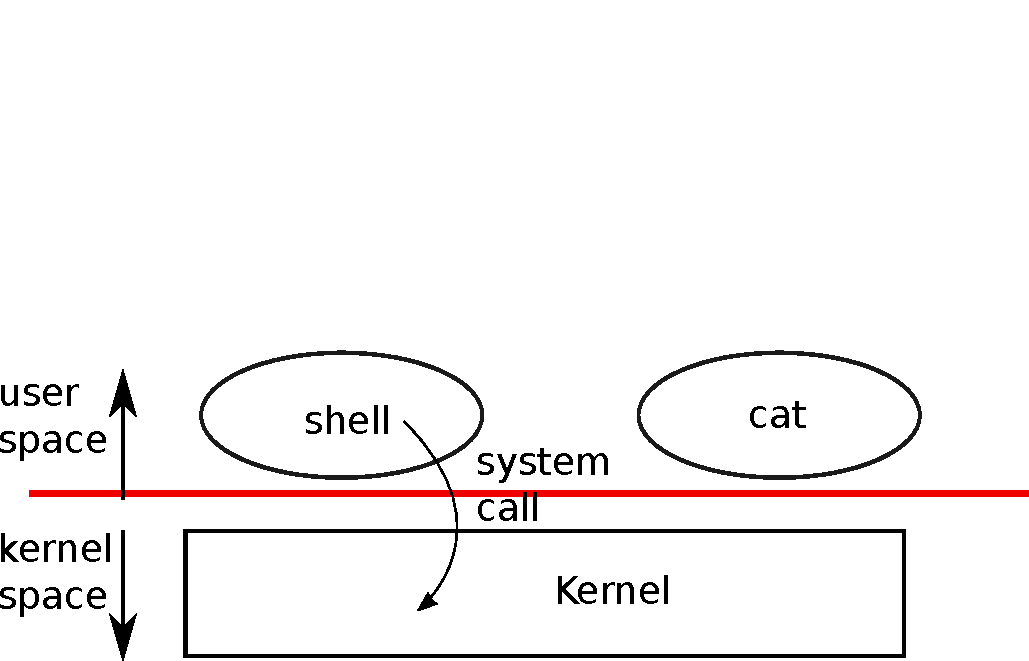
\includegraphics[scale=0.5]{fig/os.pdf}
\caption{A kernel and two user processes.}
\label{fig:os}
\end{figure}

The collection of system calls that a kernel provides
is the interface that user programs see.
The xv6 kernel provides a subset of the services and system calls
that Unix kernels traditionally offer.  
Figure~\ref{fig:api} 
lists all of xv6's system calls.

The rest of this chapter outlines xv6's services---processes, memory,
file descriptors, pipes, and a file system---and illustrates them with
code snippets and discussions of how the \indextext{shell}, which is
the primary user interface to traditional Unix-like systems, uses
them. The shell's use of system calls illustrates how carefully they
have been designed.

The shell is an ordinary program that reads commands from the user
and executes them.
The fact that the shell is a user program and not part of the kernel,
illustrates the power of the system call interface: there is nothing
special about the shell.
It also means that the shell is easy to replace; as a result,
modern Unix systems have a variety of
shells to choose from, each with its own user interface
and scripting features.
The xv6 shell is a simple implementation of the essence of
the Unix Bourne shell.  Its implementation can be found at 
\lineref{user/sh.c:1}.
%% 
%% 	Processes and memory
%% 
\section{Processes and memory}

An xv6 process consists of user-space memory (instructions, data, and stack)
and per-process state private to the kernel.
Xv6 can
\indextext{time-share} 
processes: it transparently switches the available CPUs
among the set of processes waiting to execute.
When a process is not executing, xv6 saves its CPU registers,
restoring them when it next runs the process.
The kernel associates a process identifier, or
\indexcode{pid},
with each process.

\begin{figure}[t]
\center
\begin{tabular}{ll}
{\bf System call} & {\bf Description} \\
\midrule
fork() & Create a process \\
exit(xstatus) & Terminate the current process with xstatus indicating success of failure \\
wait(*xstatus) & Wait for a child process to exit and copy the child's exit status to xstatus \\
kill(pid) & Terminate process pid \\
getpid() & Return the current process's pid \\
sleep(n) & Sleep for n clock ticks \\
exec(filename, *argv) & Load a file and execute it \\
sbrk(n) & Grow process's memory by n bytes \\
open(filename, flags) & Open a file; the flags indicate read/write \\
read(fd, buf, n) & Read n bytes from an open file into buf \\
write(fd, buf, n) & Write n bytes to an open file \\
close(fd) & Release open file fd \\
dup(fd) & Duplicate fd \\
pipe(p) & Create a pipe and return fd's in p \\
chdir(dirname) & Change the current directory \\
mkdir(dirname) & Create a new directory \\
mknod(name, major, minor) & Create a device file \\
fstat(fd) & Return info about an open file \\
link(f1, f2) & Create another name (f2) for the file f1 \\
unlink(filename) & Remove a file \\
\end{tabular}
\caption{Xv6 system calls}
\label{fig:api}
\end{figure}

A process may create a new process using the
\indexcode{fork}
system call.
\lstinline{Fork}
creates a new process, called the 
\indextext{child process}, 
with exactly the same memory contents
as the calling process, called the 
\indextext{parent process}.
\lstinline{Fork}
returns in both the parent and the child.
In the parent,
\indexcode{fork}
returns the child's pid;
in the child, it returns zero.
For example, consider the following program fragment written in the C
programming language~\cite{kernighan}:
\begin{lstlisting}[]
int pid = fork();
if(pid > 0){
  printf("parent: child=%d\n", pid);
  pid = wait(0);
  printf("child %d is done\n", pid);
} else if(pid == 0){
  printf("child: exiting\n");
  exit(0);
} else {
  printf("fork error\n");
}
\end{lstlisting}
The
\indexcode{exit}
system call causes the calling process to stop executing and
to release resources such as memory and open files.
Exit takes an integer status argument,
conventionally 0 to indicate success and 1 to indicate failure.
The
\indexcode{wait}
system call returns the pid of an exited child of the
current process and copies the exit status of the child to the address
passed to wait; if none of the caller's children
has exited,
\indexcode{wait}
waits for one to do so.
If the parent doesn't care about the exit status of a child, it can
pass a 0 address to
\lstinline{wait}.

In the example, the output lines
\begin{lstlisting}[]
parent: child=1234
child: exiting
\end{lstlisting}
might come out in either order, depending on whether the
parent or child gets to its
\indexcode{printf}
call first.
After the child exits the parent's
\indexcode{wait}
returns, causing the parent to print
\begin{lstlisting}[]
parent: child 1234 is done
\end{lstlisting}
Although the child has the same memory contents as the parent initially, the
parent and child are executing with different memory and different registers:
changing a variable in one does not affect the other. For example, when the
return value of
\lstinline{wait}
is stored into
\lstinline{pid} 
in the parent process,
it doesn't change the variable 
\lstinline{pid}
in the child.  The value of
\lstinline{pid}
in the child will still be zero.

The
\indexcode{exec}
system call
replaces the calling process's memory with a new memory
image loaded from a file stored in the file system.
The file must have a particular format, which specifies which part of
the file holds instructions, which part is data, at which instruction
to start, etc. xv6
uses the ELF format, which Chapter~\ref{CH:MEM} discusses in
more detail.
When
\indexcode{exec}
succeeds, it does not return to the calling program;
instead, the instructions loaded from the file start
executing at the entry point declared in the ELF header.
\lstinline{Exec}
takes two arguments: the name of the file containing the
executable and an array of string arguments.
For example:
\begin{lstlisting}[]
char *argv[3];

argv[0] = "echo";
argv[1] = "hello";
argv[2] = 0;
exec("/bin/echo", argv);
printf("exec error\n");
\end{lstlisting}
This fragment replaces the calling program with an instance
of the program 
\lstinline{/bin/echo}
running with the argument list
\lstinline{echo}
\lstinline{hello}.
Most programs ignore the first argument, which is 
conventionally the name of the program.

The xv6 shell uses the above calls to run programs on behalf of
users. The main structure of the shell is simple; see
\lstinline{main} 
\lineref{user/sh.c:/main/}.
The main loop reads a line of input from the user with
\indexcode{getcmd}.
Then it calls 
\lstinline{fork}, 
which creates a copy of the shell process. The
parent calls
\lstinline{wait},
while the child runs the command.  For example, if the user
had typed
``\lstinline{echo hello}''
to the shell,
\lstinline{runcmd}
would have been called with
``\lstinline{echo hello}''
as the argument.
\lstinline{runcmd} 
\lineref{user/sh.c:/runcmd/}
runs the actual command. For
``\lstinline{echo hello}'',
it would call
\lstinline{exec} 
\lineref{user/sh.c:/exec.ecmd/}.
If
\lstinline{exec}
succeeds then the child will execute instructions from
\lstinline{echo}
instead of
\lstinline{runcmd}.  
At some point
\lstinline{echo}
will call
\lstinline{exit},
which will cause the parent to return from
\lstinline{wait}
in 
\lstinline{main}
\lineref{user/sh.c:/main/}.

You might wonder why
\indexcode{fork}
and
\indexcode{exec}
are not combined in a single call; we will see later that separate
calls for creating a process and loading a program has some clever
usages in the shell for I/O redirection.  To avoid the wastefulness of
creating a duplicate process and then immediately replacing it,
operating kernels optimize the implementation of
\lstinline{fork}
for this use case by using virtual memory techniques such as
copy-on-write\mfk{need forward-reference and need to actually describe
  what COW is}.

Xv6 allocates most user-space memory
implicitly:
\indexcode{fork}
allocates the memory required for the child's copy of the
parent's memory, and 
\indexcode{exec}
allocates enough memory to hold the executable file.
A process that needs more memory at run-time (perhaps for
\indexcode{malloc})
can call
\lstinline{sbrk(n)}
to grow its data memory by
\lstinline{n}
bytes;
\indexcode{sbrk}
returns the location of the new memory.

Xv6 does not provide a notion of users or of protecting
one user from another; in Unix terms, all xv6 processes
run as root.
%% 
%% 	I/O and File descriptors
%% 
\section{I/O and File descriptors}

A 
\indextext{file descriptor} 
is a small integer representing a kernel-managed object
that a process may read from or write to.
A process may obtain a file descriptor by opening a file, directory,
or device, or by creating a pipe, or by duplicating an existing
descriptor.
For simplicity we'll often refer to the object a file descriptor
refers to as a ``file'';
the file descriptor interface abstracts away the differences between
files, pipes, and devices, making them all look like streams of bytes.
We'll refer to input and output as \indextext{I/O}.

Internally, the xv6 kernel uses the file descriptor
as an index into a per-process table,
so that every process has a private space of file descriptors
starting at zero.
By convention, a process reads from file descriptor 0 (standard input),
writes output to file descriptor 1 (standard output), and
writes error messages to file descriptor 2 (standard error).
As we will see, the shell exploits the convention to implement I/O redirection
and pipelines. The shell ensures that it always has three file descriptors
open
\lineref{user/sh.c:/open..console/},
which are by default file descriptors for the console.

The
\lstinline{read}
and
\lstinline{write}
system calls read bytes from and write bytes to
open files named by file descriptors.
The call
\lstinline{read(fd},
\lstinline{buf},
\lstinline{n)}
reads at most
\lstinline{n}
bytes from the file descriptor
\lstinline{fd},
copies them into
\lstinline{buf},
and returns the number of bytes read.
Each file descriptor that refers to a file
has an offset associated with it.
\lstinline{Read}
reads data from the current file offset and then advances
that offset by the number of bytes read:
a subsequent
\lstinline{read}
will return the bytes following the ones returned by the first
\lstinline{read}.
When there are no more bytes to read,
\lstinline{read}
returns zero to indicate the end of the file.

The call
\lstinline{write(fd},
\lstinline{buf},
\lstinline{n)}
writes
\lstinline{n}
bytes from
\lstinline{buf}
to the file descriptor
\lstinline{fd}
and returns the number of bytes written.
Fewer than
\lstinline{n}
bytes are written only when an error occurs.
Like
\lstinline{read},
\lstinline{write}
writes data at the current file offset and then advances
that offset by the number of bytes written:
each
\lstinline{write}
picks up where the previous one left off.

The following program fragment (which forms the essence of the program
\lstinline{cat})
copies data from its standard input
to its standard output.  If an error occurs, it writes a message
to the standard error.
\begin{lstlisting}[]
char buf[512];
int n;

for(;;){
  n = read(0, buf, sizeof buf);
  if(n == 0)
    break;
  if(n < 0){
    fprintf(2, "read error\n");
    exit();
  }
  if(write(1, buf, n) != n){
    fprintf(2, "write error\n");
    exit();
  }
}
\end{lstlisting}
The important thing to note in the code fragment is that
\lstinline{cat}
doesn't know whether it is reading from a file, console, or a pipe.
Similarly 
\lstinline{cat}
doesn't know whether it is printing to a console, a file, or whatever.
The use of file descriptors and the convention that file descriptor 0
is input and file descriptor 1 is output allows a simple
implementation
of 
\lstinline{cat}.

The
\lstinline{close}
system call
releases a file descriptor, making it free for reuse by a future
\lstinline{open},
\lstinline{pipe},
or
\lstinline{dup}
system call (see below).
A newly allocated file descriptor 
is always the lowest-numbered unused
descriptor of the current process.

File descriptors and
\indexcode{fork}
interact to make I/O redirection easy to implement.
\lstinline{Fork}
copies the parent's file descriptor table along with its memory,
so that the child starts with exactly the same open files as the parent.
The system call
\indexcode{exec}
replaces the calling process's memory but preserves its file table.
This behavior allows the shell to
implement \indextext{I/O redirection} by forking, reopening chosen file descriptors,
and then execing the new program.
Here is a simplified version of the code a shell runs for the
command
\lstinline{cat}
\lstinline{<}
\lstinline{input.txt}:
\begin{lstlisting}[]
char *argv[2];

argv[0] = "cat";
argv[1] = 0;
if(fork() == 0) {
  close(0);
  open("input.txt", O_RDONLY);
  exec("cat", argv);
}
\end{lstlisting}
After the child closes file descriptor 0,
\lstinline{open}
is guaranteed to use that file descriptor
for the newly opened
\lstinline{input.txt}:
0 will be the smallest available file descriptor.
\lstinline{Cat}
then executes with file descriptor 0 (standard input) referring to
\lstinline{input.txt}.

The code for I/O redirection in the xv6 shell works in exactly this way
\lineref{user/sh.c:/case.REDIR/}.
Recall that at this point in the code the shell has already forked the
child shell and that 
\lstinline{runcmd} 
will call
\lstinline{exec}
to load the new program.  Now it should be clear why it is a good idea that
\lstinline{fork}
and 
\lstinline{exec} 
are separate calls.  Because if they are separate, the shell can fork a child,
use
\lstinline{open},
\lstinline{close},
\lstinline{dup}
in the child to change the standard input and output
file descriptors, and then
\lstinline{exec}.
No changes to the program being exec-ed
(\lstinline{cat}
in our example)
are required.
If
\lstinline{fork}
and
\lstinline{exec}
were combined into a single
system call, some other (probably more complex) scheme would be required for the
shell to redirect standard input and output, or the program itself would have to
understand how to redirect I/O.

Although
\lstinline{fork}
copies the file descriptor table, each underlying file offset is shared
between parent and child.
Consider this example:
\begin{lstlisting}[]
if(fork() == 0) {
  write(1, "hello ", 6);
  exit(0);
} else {
  wait(0);
  write(1, "world\n", 6);
}
\end{lstlisting}
At the end of this fragment, the file attached to file descriptor 1
will contain the data
\lstinline{hello}
\lstinline{world}.
The
\lstinline{write}
in the parent
(which, thanks to
\lstinline{wait},
runs only after the child is done)
picks up where the child's
\lstinline{write}
left off.
This behavior helps produce sequential output from sequences
of shell commands, like
\lstinline{(echo}
\lstinline{hello};
\lstinline{echo}
\lstinline{world)}
\lstinline{>output.txt}.

The
\lstinline{dup}
system call duplicates an existing file descriptor,
returning a new one that refers to the same underlying I/O object.
Both file descriptors share an offset, just as the file descriptors
duplicated by
\lstinline{fork}
do.
This is another way to write
\lstinline{hello}
\lstinline{world}
into a file:
\begin{lstlisting}[]
fd = dup(1);
write(1, "hello ", 6);
write(fd, "world\n", 6);
\end{lstlisting}

Two file descriptors share an offset if they were derived from
the same original file descriptor by a sequence of
\lstinline{fork}
and
\lstinline{dup}
calls.
Otherwise file descriptors do not share offsets, even if they
resulted from 
\lstinline{open}
calls for the same file.  
\lstinline{Dup} 
allows shells to implement commands like this:
\lstinline{ls}
\lstinline{existing-file}
\lstinline{non-existing-file}
\lstinline{>}
\lstinline{tmp1}
\lstinline{2>&1}.
The
\lstinline{2>&1}
tells the shell to give the command a file descriptor 2 that
is a duplicate of descriptor 1.
Both the name of the existing file and the error message for the
non-existing file will show up in the file
\lstinline{tmp1}.
The xv6 shell doesn't support I/O redirection for the error file
descriptor, but now you know how to implement it.

File descriptors are a powerful abstraction,
because they hide the details of what they are connected to:
a process writing to file descriptor 1 may be writing to a
file, to a device like the console, or to a pipe.
%% 
%% 	Pipes
%% 
\section{Pipes}

A 
\indextext{pipe} 
is a small kernel buffer exposed to processes as a pair of
file descriptors, one for reading and one for writing.
Writing data to one end of the pipe
makes that data available for reading from the other end of the pipe.
Pipes provide a way for processes to communicate.

The following example code runs the program
\lstinline{wc}
with standard input connected to
the read end of a pipe.
\begin{lstlisting}[]
int p[2];
char *argv[2];

argv[0] = "wc";
argv[1] = 0;

pipe(p);
if(fork() == 0) {
  close(0);
  dup(p[0]);
  close(p[0]);
  close(p[1]);
  exec("/bin/wc", argv);
} else {
  close(p[0]);
  write(p[1], "hello world\n", 12);
  close(p[1]);
}
\end{lstlisting}
The program calls
\lstinline{pipe},
which creates a new pipe and records the read and write
file descriptors in the array
\lstinline{p}.
After
\lstinline{fork},
both parent and child have file descriptors referring to the pipe.
The child dups the read end onto file descriptor 0,
closes the file descriptors in
\lstinline{p},
and execs
\lstinline{wc}.
When 
\lstinline{wc}
reads from its standard input, it reads from the pipe.
The parent closes the read side of the pipe,
writes to the pipe,
and then closes the write side.

If no data is available, a
\lstinline{read}
on a pipe waits for either data to be written or all
file descriptors referring to the write end to be closed;
in the latter case,
\lstinline{read}
will return 0, just as if the end of a data file had been reached.
The fact that
\lstinline{read}
blocks until it is impossible for new data to arrive
is one reason that it's important for the child to
close the write end of the pipe
before executing
\lstinline{wc}
above: if one of
\lstinline{wc} 's
file descriptors referred to the write end of the pipe,
\lstinline{wc}
would never see end-of-file.

The xv6 shell implements pipelines such as
\lstinline{grep fork sh.c | wc -l}
in a manner similar to the above code
\lineref{user/sh.c:/case.PIPE/}.
The child process creates a pipe to connect the left end of the pipeline
with the right end. Then it calls
\lstinline{fork}
and
\lstinline{runcmd}
for the left end of the pipeline
and 
\lstinline{fork}
and
\lstinline{runcmd}
for the right end, and waits for both to finish.
The right end of the pipeline may be a command that itself includes a
pipe (e.g.,
\lstinline{a}
\lstinline{|}
\lstinline{b}
\lstinline{|}
\lstinline{c)}, 
which itself forks two new child processes (one for
\lstinline{b}
and one for
\lstinline{c}).
Thus, the shell may
create a tree of processes.  The leaves of this tree are commands and
the interior nodes are processes that wait until the left and right
children complete.

In principle, one could have the interior nodes run the left end of a
pipeline, but doing so correctly would complicate the
implementation. Consider making just the following modification:
change \lstinline{sh.c} to not fork for \lstinline{p->left} and run
\lstinline{runcmd(p->left)} in the interior process. Then, for
example, \lstinline{echo hi | wc} won't produce output, because when
\lstinline{echo hi} exits in \lstinline{runcmd}, the interior process
exits and never calls fork to run the right end of the pipe.  This
incorrect behavior could be fixed by not calling \lstinline{exit} in
\lstinline{runcmd} for interior processes, but this fix complicates
the code: now \lstinline{runcmd} needs to know if it a interior
process or not.  Complications also arise when not forking for
\lstinline{runcmd(p->right)}.  For example, with just that modification,
\lstinline{sleep 10 | echo hi} will immediately print ``hi'' instead
of after 10 seconds, because \lstinline{echo} runs immediately and
exits, not waiting for \lstinline{sleep} to finish.  Since the goal of
the \lstinline{sh.c} is to be as simple as possible, it doesn't try to
avoid creating interior processes.

Pipes may seem no more powerful than temporary files:
the pipeline
\begin{lstlisting}[]
echo hello world | wc
\end{lstlisting}
could be implemented without pipes as
\begin{lstlisting}[]
echo hello world >/tmp/xyz; wc </tmp/xyz
\end{lstlisting}
Pipes have at least four advantages over temporary files
in this situation.
First, pipes automatically clean themselves up;
with the file redirection, a shell would have to
be careful to remove
\lstinline{/tmp/xyz}
when done.
Second, pipes can pass arbitrarily long streams of
data, while file redirection requires enough free space
on disk to store all the data.
Third, pipes allow for parallel execution of pipeline stages,
while the file approach requires the first program to finish
before the second starts.
Fourth, if you are implementing inter-process communication,
pipes' blocking reads and writes are more efficient
than the non-blocking semantics of files.
%% 
%% 	File system
%% 
\section{File system}

The xv6 file system provides data files,
which are uninterpreted byte arrays,
and directories, which
contain named references to data files and other directories.
The directories form a tree, starting
at a special directory called the 
\indextext{root}.
A 
\indextext{path} 
like
\lstinline{/a/b/c}
refers to the file or directory named
\lstinline{c}
inside the directory named
\lstinline{b}
inside the directory named
\lstinline{a}
in the root directory
\lstinline{/}.
Paths that don't begin with
\lstinline{/}
are evaluated relative to the calling process's
\indextext{current directory},
which can be changed with the
\lstinline{chdir}
system call.
Both these code fragments open the same file
(assuming all the directories involved exist):
\begin{lstlisting}[]
chdir("/a");
chdir("b");
open("c", O_RDONLY);

open("/a/b/c", O_RDONLY);
\end{lstlisting}
The first fragment changes the process's current directory to
\lstinline{/a/b};
the second neither refers to nor changes the process's current directory.

There are multiple system calls to create a new file or directory:
\lstinline{mkdir}
creates a new directory,
\lstinline{open}
with the
\lstinline{O_CREATE}
flag creates a new data file,
and
\lstinline{mknod}
creates a new device file.
This example illustrates all three:
\begin{lstlisting}[]
mkdir("/dir");
fd = open("/dir/file", O_CREATE|O_WRONLY);
close(fd);
mknod("/console", 1, 1);
\end{lstlisting}
\lstinline{Mknod}
creates a file in the file system,
but the file has no contents.
Instead, the file's metadata marks it as a device file
and records the major and minor device numbers
(the two arguments to 
\lstinline{mknod}),
which uniquely identify a kernel device.
When a process later opens the file, the kernel
diverts
\lstinline{read}
and
\lstinline{write}
system calls to the kernel device implementation
instead of passing them to the file system.

\lstinline{Fstat}
retrieves information about the object a file
descriptor refers to.
It fills in a
\lstinline{struct}
\lstinline{stat},
defined in
\lstinline{stat.h} \fileref{kernel/stat.h}
as:
\begin{lstlisting}[]
#define T_DIR     1   // Directory
#define T_FILE    2   // File
#define T_DEVICE  3   // Device

struct stat {
  int dev;     // File system's disk device
  uint ino;    // Inode number
  short type;  // Type of file
  short nlink; // Number of links to file
  uint64 size; // Size of file in bytes
};
\end{lstlisting}

A file's name is distinct from the file itself;
the same underlying file, called an 
\indextext{inode}, 
can have multiple names,
called 
\indextext{links}.
The
\lstinline{link}
system call creates another file system name 
referring to the same inode as an existing file.
This fragment creates a new file named both
\lstinline{a}
and
\lstinline{b}.
\begin{lstlisting}[]
open("a", O_CREATE|O_WRONLY);
link("a", "b");
\end{lstlisting}
Reading from or writing to
\lstinline{a}
is the same as reading from or writing to
\lstinline{b}.
Each inode is identified by a unique
\textit{inode}
\textit{number}.
After the code sequence above, it is possible
to determine that
\lstinline{a}
and
\lstinline{b}
refer to the same underlying contents by inspecting the
result of 
\lstinline{fstat}:
both will return the same inode number 
(\lstinline{ino}),
and the
\lstinline{nlink}
count will be set to 2.

The
\lstinline{unlink}
system call removes a name from the file system.
The file's inode and the disk space holding its content
are only freed when the file's link count is zero and
no file descriptors refer to it.
Thus adding
\begin{lstlisting}[]
unlink("a");
\end{lstlisting}
to the last code sequence leaves the inode
and file content accessible as
\lstinline{b}.
Furthermore,
\begin{lstlisting}[]
fd = open("/tmp/xyz", O_CREATE|O_RDWR);
unlink("/tmp/xyz");
\end{lstlisting}
is an idiomatic way to create a temporary inode 
that will be cleaned up when the process closes 
\lstinline{fd}
or exits.

Shell commands for file system operations are implemented
as user-level programs such as
\lstinline{mkdir},
\lstinline{ln},
\lstinline{rm},
etc. This design allows anyone to extend the shell with new user commands by
just adding a new user-level program.  In hindsight this plan seems obvious,
but other systems designed at the time of Unix often built such commands into
the shell (and built the shell into the kernel).

One exception is
\lstinline{cd},
which is built into the shell
\lineref{user/sh.c:/if.buf.0..==..c./}.
\lstinline{cd}
must change the current working directory of the
shell itself.  If
\lstinline{cd}
were run as a regular command, then the shell would fork a child
process, the child process would run
\lstinline{cd},
and
\lstinline{cd}
would change the 
\textit{child} 's 
working directory.  The parent's (i.e.,
the shell's) working directory would not change.
%% 
%% 	Real world
%% 
\section{Real world}

Unix's combination of ``standard'' file
descriptors, pipes, and convenient shell syntax for
operations on them was a major advance in writing
general-purpose reusable programs.
The idea sparked a whole culture of ``software tools'' that was
responsible for much of Unix's power and popularity,
and the shell was the first so-called ``scripting language.''
The Unix system call interface persists today in systems like
BSD, Linux, and Mac OS X.

The Unix system call interface has been standardized through the Portable
Operating System Interface (POSIX) standard.
Xv6 is
\textit{not}
POSIX compliant.  It misses system calls (including basic ones such as
\lstinline{lseek}),
it implements system calls only partially, as well as other differences.  Our main goals for xv6 are
simplicity and clarity while providing a simple UNIX-like system-call interface.
Several people have extended xv6 with a few more system calls and a simple
C library in order to run basic Unix programs.  Modern kernels, however,
provide many more system calls, and many more kinds of kernel services, than
xv6.  For example, they support networking, windowing systems, user-level threads,
drivers for many devices, and so on.  Modern kernels evolve continuously and
rapidly, and offer many features beyond POSIX.

For the most part, modern Unix-derived operating systems
have not followed the early
Unix model of exposing devices as special files, like the
\lstinline{console}
device file discussed above.
The authors of Unix went on to build Plan 9,
which applied the ``resources are files''
concept to modern facilities,
representing networks, graphics, and other resources
as files or file trees.

The file system and file descriptors have been  powerful
abstractions.
Even so, there are other models for operating system interfaces.
Multics, a predecessor of Unix,
abstracted file storage in a way that made it look like memory,
producing a very different flavor of interface.
The complexity of the Multics design had a direct influence
on the designers of Unix, who tried to build something simpler.
% XXX can we cut this, since its point is the same as the next paragraph?
% An operating system interface that went out of fashion
% decades ago but has recently returned is the idea of a virtual machine monitor.
% Such systems provide a superficially different interface from xv6,
% but the basic concepts are still the same:
% a virtual machine, like a process, consists of some memory and
% one or more register sets;
% the virtual machine has access to one large file called
% a virtual disk instead of a file system;
% virtual machines send messages to each other
% and the outside world using virtual network devices
% instead of pipes or files.

This book examines how xv6 implements its Unix-like interface,
but the ideas and concepts apply to more than just Unix.
Any operating system must multiplex processes onto
the underlying hardware, isolate processes from each
other, and provide mechanisms for controlled
inter-process communication.
After studying xv6, you should be able to
look at other, more complex operating systems
and see the concepts underlying xv6 in those systems as well.

%% 
\section{Exercises}
%%

\begin{enumerate}

\item Write a program that uses UNIX system calls to
``ping-pong'' a byte between two processes over a pair
of pipes, one for each direction. Measure the
program's performance, in exchanges per second.

\end{enumerate}

%   terminology:
%     process: refers to execution in user space, or maybe struct proc &c
%     process memory: the lower part of the address space
%     process has one thread with two stacks (one for in kernel mode and one for
%     in user mode)
% talk a little about initial page table conditions:
%     paging not on, but virtual mostly mapped direct to physical,
%     which is what things look like when we turn paging on as well
%     since paging is turned on after we create first process.
%   mention why still have SEG_UCODE/SEG_UDATA?
%   do we ever really say what the low two bits of %cs do?
%     in particular their interaction with PTE_U
%   sidebar about why it is extern char[]

\chapter{Operating system organization}
\label{CH:FIRST}

A key requirement for an operating system is to support several activities at once.  For
example, using the system call interface described in
chapter~\ref{CH:UNIX}
a process can start new processes with 
\lstinline{fork}.
The operating system must 
\indextext{time-share} 
the resources of the computer among these processes.
For example, even if there are more processes
than there are hardware CPUs, the operating
system must ensure that all of the processes
make progress.  The operating system must also arrange for
\indextext{isolation} 
between the processes.
That is, if one process has a bug and fails, it shouldn't affect processes that
don't depend on the failed process.
Complete isolation, however, is too strong, since it should be possible for
processes to intentionally interact; pipelines are an example.
Thus
an operating system must fulfill three requirements: multiplexing, isolation,
and interaction.

This chapter provides an overview of how operating systems are
organized to achieve these three requirements.  It turns out there are
many ways to do so, but this text focuses on mainstream designs
centered around a \indextext{monolithic kernel}, which is used by many
Unix operating systems.  This chapter also provides an overview of an
xv6 process, which is the unit of isolation in xv6, and the
creation of the first process when xv6 starts running.

Xv6 runs on a RISC-V development board, and much of its low-level
functionality (for example, its process implementation) is specific to
RISC-V.  RISC-V is a 64-bit CPU, and xv6 is written in ``LP64'' C,
which means long (L) and pointers (P) in the C programming language
are 64 bits, but int is 32-bit.  This book assumes the reader has done
a bit of machine-level programming on some architecture, and will
introduce RISC-V-specific ideas as they come up.  A useful reference
for RISC-V is ``The RISC-V Reader: An Open Architecture
Atlas''~\cite{riscv}.
The user-level ISA~\cite{riscv:user} and the privileged
architecture~\cite{riscv:priv} are the official specifications.

This text generally refers to the hardware element that executes a
computation with the term \indextext{CPU}, an acronym for central
processing unit.  Other documentation (e.g., RISC-V specifications)
also uses the words processor, core, and hart instead of CPU.  Related
terms are \indextext{multicore processor} (a single chip with several
CPUs on it) and \indextext{multiprocessor} (a computer board with
several processor chips).

%% 
\section{Abstracting physical resources}
%% 

The first question one might ask when encountering an operating system is why
have it at all?  That is, one could implement the system calls in
Figure~\ref{fig:api}
as a library, with which applications link.  In this plan,
each application could even have its own library tailored to its needs.
Applications could directly interact with hardware resources
and use those resources in the best way for the application (e.g., to achieve
high or predictable performance).  Some operating systems for
embedded devices or real-time systems are organized in this way.

The downside of this library approach is that, if there is more than one
application running, the applications must be well-behaved.
For example, each application must periodically give up the
CPU so that other applications can run.
Such a 
\textit{cooperative} 
time-sharing scheme may be OK if all applications trust each
other and have no bugs. It's more typical for applications
to not trust each other, and to have bugs, so one often wants
stronger isolation than a cooperative scheme provides.

To achieve strong isolation it's helpful to forbid applications from
directly accessing sensitive hardware resources, and instead to abstract the
resources into services.  For example, applications interact with a file system
only through
\lstinline{open},
\lstinline{read},
\lstinline{write}, 
and
\lstinline{close}
system calls,
instead of read and writing raw disk sectors. 
This provides the application with the convenience of pathnames, and it allows
the operating system (as the implementer of the interface) to manage the disk. 

Similarly, Unix transparently switches hardware CPUs among processes,
saving and restoring register state as necessary,
so that applications don't have to be
aware of time sharing.  This transparency allows the operating system to share
CPUs even if some applications are in infinite loops.

As another example, Unix processes use 
\lstinline{exec}
to build up their memory image, instead of directly interacting with physical
memory.  This allows the operating system to decide where to place a process in
memory; if memory is tight, the operating system might even store some of
a process's data on disk.
\lstinline{Exec}
also provides
users with the convenience of a file system to store executable program images.  

Many forms of interaction among Unix processes occur via file descriptors.
Not only do file descriptors abstract away many details (e.g.,
where data in a pipe or file is stored), they also are defined in a
way that simplifies interaction.
For example, if one application in a pipeline fails, the kernel
generates end-of-file for the next process in the pipeline.

As you can see, the system call interface in
Figure~\ref{fig:api}
is carefully designed to provide both programmer convenience and
the possibility of strong isolation.  The Unix interface
is not the only way to abstract resources, but it has proven to be a very good
one.

%% 
\section{User mode, supervisor mode, and system calls}
%% 

Strong isolation requires a hard boundary between applications and the operating
system.  If the application makes a mistake, we don't want the operating system
to fail or other applications to fail. Instead, the operating system should be
able to clean up the failed application and continue running other applications.
To achieve strong isolation, the operating system must arrange that applications cannot modify (or even
read) the operating system's data structures and instructions and that
applications cannot access other process's memory.

CPUs provide hardware support for strong isolation.   For
example, RISC-V has three modes in which
the CPU can execute instructions:
\indextext{machine mode},
\indextext{supervisor mode}, and
\indextext{user mode}.
Instructions executing in machine mode have full privilege; a
CPU starts in machine mode.  Machine mode is mostly intended for
configuring a computer.  Xv6 executes a few lines in machine mode and
then changes to supervisor mode.

In supervisor mode the CPU is allowed to execute 
\indextext{privileged instructions}.
For example, enabling and disabling interrupts,  reading and writing
the register that holds the address of a page table, etc.
If an application in user mode attempts to execute
a privileged instruction, then the CPU doesn't execute the instruction, but switches
to supervisor mode so that supervisor-mode code can terminate the application,
because it did something it shouldn't be doing. 
Figure~\ref{fig:os}
in Chapter ~\ref{CH:UNIX} illustrates this organization.  An application can
execute only user-mode instructions (e.g., adding numbers, etc.) and is said to
be running in 
\indextext{user space},
while the software in supervisor mode can also execute privileged instructions and
is said to be running in
\indextext{kernel space}.
The software running in kernel space (or in supervisor mode) is called
the
\indextext{kernel}.

An application that wants to invoke a kernel function (e.g., the
\lstinline{read}
system call in xv6) must to
transition to the kernel.  CPUs provide a special instruction that switches the
CPU from user mode to supervisor mode and enters the kernel at an entry point
specified by the kernel.  (RISC-V
provides the 
\indexcode{ecall}
instruction for this purpose.)  Once the CPU has switched to supervisor mode,
the kernel can then validate the arguments of the system call, decide whether
the application is allowed to perform the requested operation, and then deny it
or execute it.  It is important that the kernel control the entry point for
transitions to supervisor mode; if the application could decide the kernel entry
point, a malicious application could enter the kernel at a point where the
validation of arguments etc. is skipped.
%% 
\section{Kernel organization}
%% 

A key design question is what part of the operating
system should run in supervisor mode. 
One possibility is that the entire operating system resides
in the kernel, so that the implementations of all system calls
run in supervisor mode.
This organization is called a
\indextext{monolithic kernel}.

In this organization the entire operating system runs with full hardware
privilege. This organization is convenient because the OS designer doesn't have
to decide which part of the operating system doesn't need full hardware
privilege.  Furthermore, it easy for different parts of the operating system to
cooperate.  For example, an operating system might have a buffer cache that can
be shared both by the file system and the virtual memory system. 

A downside of the monolithic organization is that the interfaces between
different parts of the operating system are often complex (as we will see in the
rest of this text), and therefore it is easy for an operating system developer
to make a mistake.  In a monolithic kernel, a mistake is fatal, because an error
in supervisor mode will often cause the kernel to fail.  If the kernel fails,
the computer stops working, and thus all applications fail too.  The computer
must reboot to start again.

To reduce the risk of mistakes in the kernel, OS designers can minimize the
amount of operating system code that runs in supervisor mode, and execute the
bulk of the operating system in user mode.
This kernel organization is called a
\indextext{microkernel}.

\begin{figure}[t]
\center
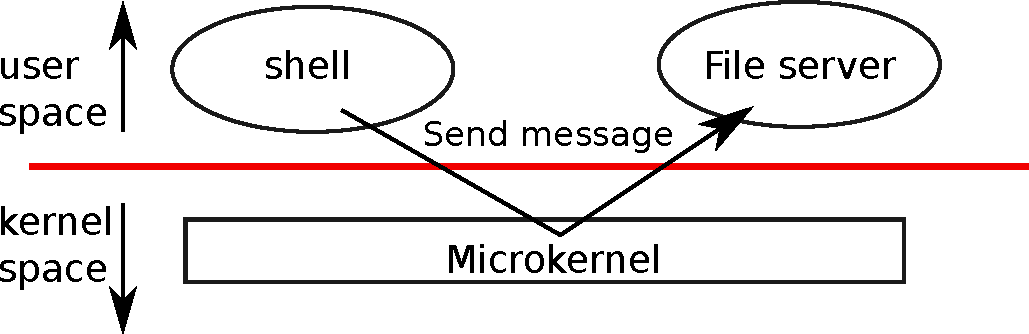
\includegraphics[scale=0.5]{fig/mkernel.pdf}
\caption{A microkernel with a file system server}
\label{fig:mkernel}
\end{figure}

Figure~\ref{fig:mkernel}
illustrates this microkernel design.  In the figure, the file system runs as a
user-level process.  OS services running as processes are called servers.
To allow applications to interact with the
file server, the kernel provides an inter-process communication
mechanism to send messages from one
user-mode process to another.  For example, if an application like the shell
wants to read or write a file, it sends a message to the file server and waits
for a response. 

In a microkernel, the kernel interface consists of a few low-level
functions for starting applications, sending messages,
accessing device hardware, etc.  This organization allows the kernel to be 
relatively simple, as most of the operating system
resides in user-level servers.

Xv6 is
implemented as a monolithic kernel, like most Unix operating systems.
Thus, the xv6 kernel interface corresponds to the operating system
interface, and the kernel implements the complete operating system.  Since 
xv6 doesn't provide many services, its kernel is smaller than some
microkernels, but conceptually xv6 is monolithic.
%% 
\section{Process overview}
%% 

The unit of isolation in xv6 (as in other Unix operating systems) is a 
\indextext{process}.
The process abstraction prevents one process from wrecking or spying on
another process's memory, CPU, file descriptors, etc.  It also prevents a process
from wrecking the kernel itself, so that a process can't subvert the kernel's
isolation mechanisms.
The kernel must implement the process abstraction with care because
a buggy or malicious application may trick the kernel or hardware in doing
something bad (e.g., circumventing isolation).  The mechanisms used by
the kernel to implement processes include the user/supervisor mode flag, address spaces,
and time-slicing of threads.

To help enforce isolation, the process abstraction provides the
illusion to a program that it has its own private machine.  A process provides
a program with what appears to be a private memory system, or
\indextext{address space}, 
which other processes cannot read or write.
A process also provides the program with what appears to be its own
CPU to execute the program's instructions.

Xv6 uses page tables (which are implemented by hardware) to give each process
its own address space. The RISC-V page table
translates (or ``maps'') a
\indextext{virtual address}
(the address that an RISC-V instruction manipulates) to a
\indextext{physical address}
(an address that the CPU chip sends to main memory).

\begin{figure}[t]
\center
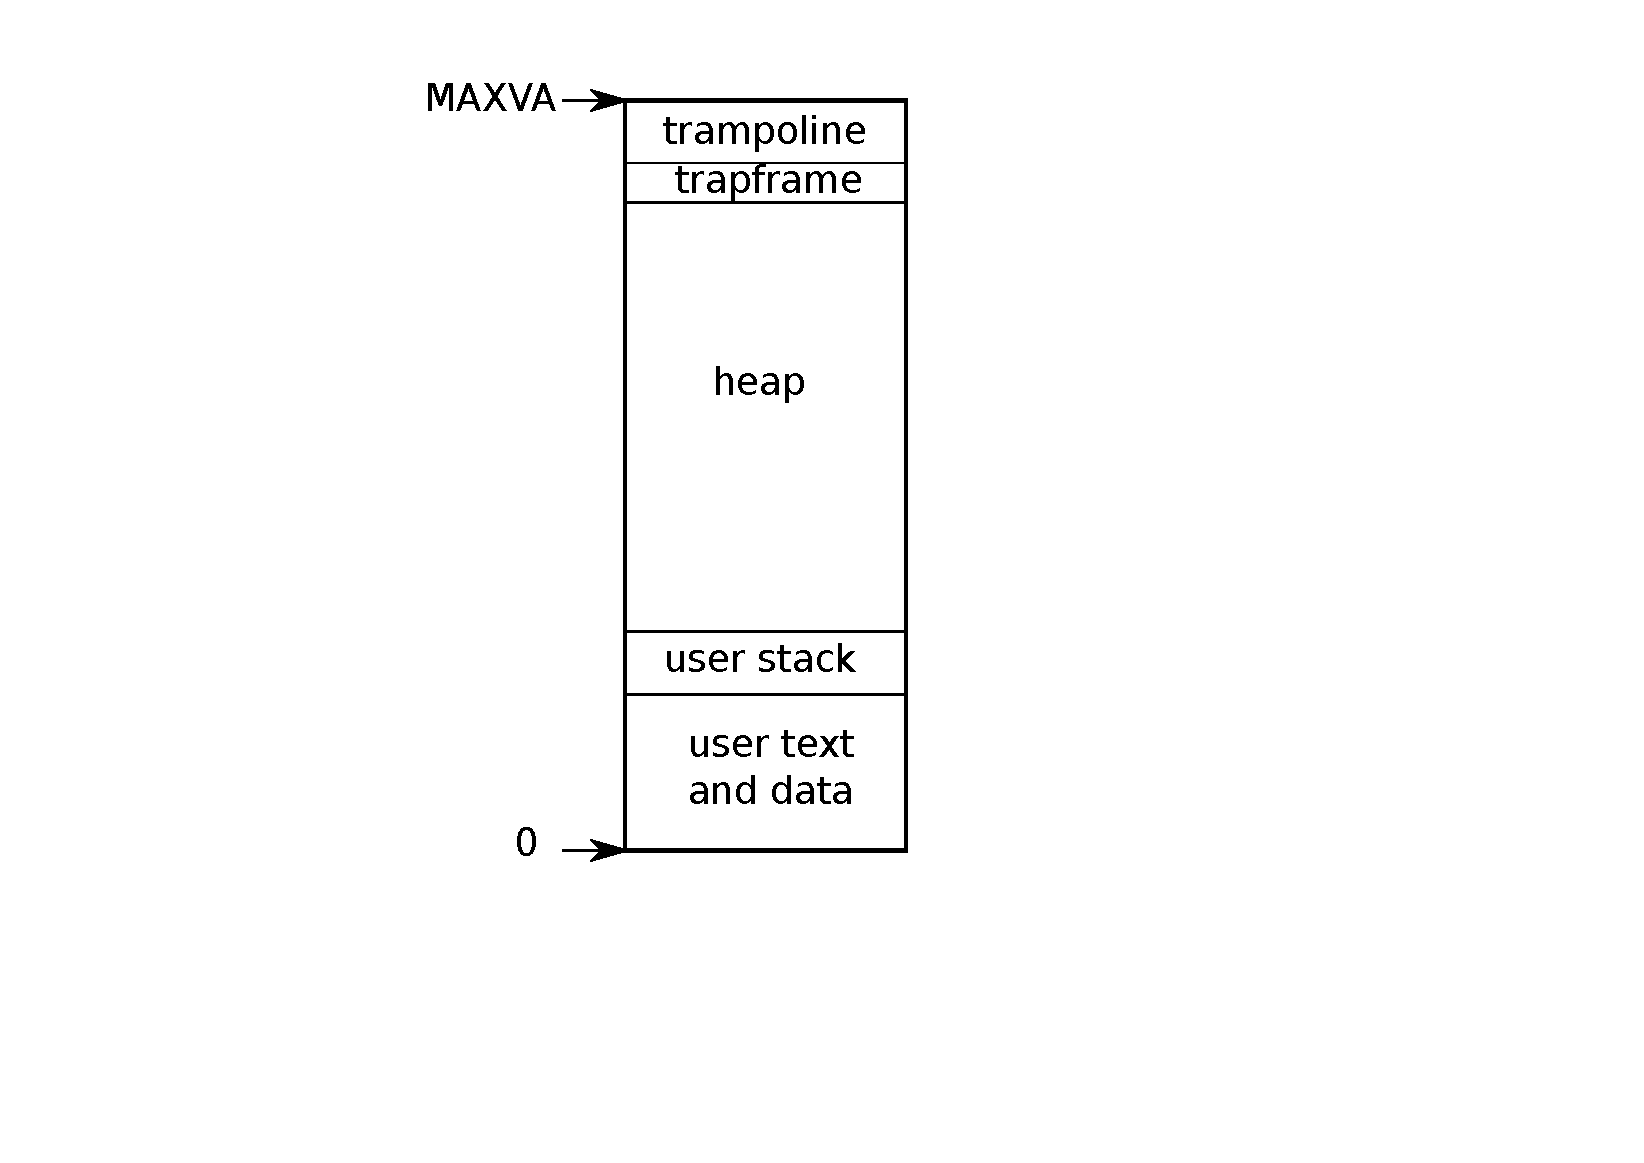
\includegraphics[scale=0.5]{fig/as.pdf}
\caption{Layout of a virtual address space of a user process}
\label{fig:as}
\end{figure}

Xv6 maintains a separate page table for each process that defines that process's
address space. As illustrated in 
Figure~\ref{fig:as},
an address space includes the process's
\indextext{user memory}
starting at virtual address zero. Instructions come first,
followed by global variables, then the stack,
and finally a ``heap'' area (for malloc)
that the process can expand as needed.
Xv6 runs on RISC-V with 39 bits for virtual addresses,
but uses only 38 bits.  Thus, the maximum address is $2^{38}-1$ =
0x3fffffffff, which is \lstinline{MAXVA}~\lineref{kernel/riscv.h:/MAXVA/}.
At the top of the address space xv6 reserves a page
for a \indextext{trampoline} and a page mapping
the process's \indextext{trapframe}
to switch to the kernel, as we will explain in Chapter~\ref{CH:TRAP}.

The xv6 kernel maintains many pieces of state for each process,
which it gathers into a
\indexcode{struct proc}
\lineref{kernel/proc.h:/^struct.proc/}.
A process's most important pieces of kernel state are its 
page table, its kernel stack, and its run state.
We'll use the notation
\indexcode{p->xxx}
to refer to elements of the
\lstinline{proc}
structure.  The trapframe mentioned above is \indexcode{p->tf}.

Each process has a thread of execution (or 
\indextext{thread}
for short) that executes the process's instructions.
A thread can be suspended and later resumed.
To switch transparently between processes,
the kernel suspends the currently running thread and resumes another process's
thread.  Much of the state of a thread (local variables, function call return
addresses) is stored on the thread's stacks.
Each process has two stacks: a user stack and a kernel stack
(\indexcode{p->kstack}).
When the process is executing user instructions, only its user stack
is in use, and its kernel stack is empty.
When the process enters the kernel (for a system call or interrupt),
the kernel code executes on the process's kernel stack; while
a process is in the kernel, its user stack still contains saved
data, but isn't actively used.
A process's thread alternates between actively using its user stack
and its kernel stack. The kernel stack is separate (and protected from
user code) so that the kernel
can execute even if a process has wrecked its user stack.

A process can make a system call by executing the RISC-V \indexcode{ecall}
instruction. This instruction raises the hardware privilege level and
changes the program counter to a kernel-defined entry point.  The code
at the entry point switches to a kernel stack and executes the kernel
instructions that implement the system call.  When the system call
completes, the kernel switches back to the user stack and returns to
user space by calling the \indexcode{sret} instruction, which lowers
the hardware privilege level and resumes executing user instructions
just after the system call instruction.  A process's thread can
``block'' in the kernel to wait for I/O, and resume where it left off
when the I/O has finished.

\indexcode{p->state} 
indicates whether the process is allocated, ready
to run, running, waiting for I/O, or exiting.

\indexcode{p->pagetable}
holds the process's page table, in the format
that the RISC-V hardware expects.
xv6 causes the paging hardware to use a process's
\lstinline{p->pagetable}
when executing that process in user space.
A process's page table also serves as the record of the
addresses of the physical pages allocated to store the process's memory.
%% 
\section{Code: starting xv6 and the first process}
%% 
To make xv6 more concrete, we'll outline how the kernel starts and
runs the first process. The subsequent chapters will describe the
mechanisms that show up in this overview in more detail.

When the RISC-V development board powers on, it initializes
itself and runs a boot loader which is stored in read-only
memory.  The boot loader loads the xv6 kernel into memory.  Then, in
machine mode, the CPU executes xv6 starting at
\indexcode{\_entry}
\lineref{kernel/entry.S:/^.entry:/}.
Xv6 starts with the RISC-V paging hardware disabled:
virtual addresses map directly to physical addresses.

The loader loads the xv6 kernel into memory at physical address
\texttt{0x80000000}.
The reason it places the kernel at
\texttt{0x80000000}
rather than
\texttt{0x0}
is because the address range
\texttt{0x0:0x80000000}
contains I/O devices.

The instructions at
\lstinline{_entry}
set up a stack so that xv6 can run C code.
xv6 declares space for an initial stack,
\lstinline{stack0},
in the file
\lstinline{start.c}
\lineref{kernel/start.c:/stack0/}.
The code at
\lstinline{_entry}
loads the stack pointer register
\texttt{sp}
with the address
\lstinline{stack0+4096},
the top of the stack, because the stack
on RISC-V grows down.
Now that we have a stack,
\lstinline{_entry}
calls into C code at
\lstinline{start}
\lineref{kernel/start.c:/^start/}.

The function
\lstinline{start}
performs some configuration that is only allowed in
machine mode, and then switches to supervisor mode.
To enter supervisor mode, RISC-V
provides the instruction
\lstinline{mret}.
This instruction is most often used to return from
a previous call from supervisor mode to machine mode.
\lstinline{start} isn't returning from such a call, and
instead sets things up as if there had been one:
it sets the previous privilege mode to
supervisor in the register
\lstinline{mstatus},
it sets the return address to
\lstinline{main}
by writing
\lstinline{main}'s
address into
the register
\lstinline{mepc},
disables virtual memory in supervisor mode
by writing
\lstinline{0}
into the page-table register
\lstinline{satp},
and delegates all interrupts and exceptions
to supervisor mode.

Before jumping into supervisor mode,
\lstinline{start}
performs one more task: it programs the clock
chip to generate timer interrupts.
With this housekeeping out of the way,
\lstinline{start}
``returns'' to supervisor
mode by calling
\lstinline{mret}.
This causes the program counter to change
to
\lstinline{main}
\lineref{kernel/main.c:/^main/}.

After
\lstinline{main}
\lineref{kernel/main.c:/^main/}  
initializes several devices and subsystems, 
it creates the first process by calling 
\lstinline{userinit}
\lineref{kernel/proc.c:/^userinit/}.
The first process executes a small program,
\indexcode{initcode.S} 
\lineref{user/initcode.S:1},
which re-enters the kernel by invoking the
\lstinline{exec}
system call.
As we saw in Chapter~\ref{CH:UNIX}, 
\indexcode{exec}
replaces the memory and registers of the
current process with a new program (in this case,
\lstinline{/init}).
Once the kernel has completed 
\lstinline{exec},
it returns to user space and runs
\indexcode{/init}.
\lstinline{Init}
\lineref{user/init.c:/^main/}
creates a new console device file
if needed
and then opens it as file descriptors 0, 1, and 2.
Then it loops,
starting a console shell, 
handles orphaned zombies until the shell exits,
and repeats.
The system is up.
%% 
\section{Real world}
%% 

In the real world, one can find both monolithic kernels and microkernels. Many
Unix kernels are monolithic. For example, Linux has a monolithic kernel,
although some OS functions run as user-level servers (e.g., the windowing
system).  Kernels such as L4, Minix, QNX are organized as a microkernel with
servers, and have seen wide deployment in embedded settings.

Most operating systems have adopted the process concept, and most
processes look similar to xv6's.  Modern operating systems, however,
support several threads within a process, to allow a single process to
exploit multiple CPUs.  Supporting multiple threads in a
process involves quite a bit of machinery that xv6 doesn't have,
including potential interface changes (e.g., Linux's
\lstinline{clone},
a variant of
\lstinline{fork}),
to control which parts of
a process threads share.
%% 
\section{Exercises}
%%

\begin{enumerate}
  
\item Set a breakpoint at \lstinline{swtch}.  Single step with gdb's
\lstinline{stepi}
through the ret to
\lstinline{forkret},
then use gdb's
\lstinline{finish}
to proceed to
\lstinline{usertrapret},
then
\lstinline{stepi}
until you get to
\lstinline{initcode} 
at virtual address zero.

\end{enumerate}


{
% The following prevents latex from splitting a bibliography entry with a page
% break
\interlinepenalty=10000
% Since we're using natbib in numbers mode, we don't need plainnat,
% which exists to feed authors and years back in to natbib.  As a
% result, it complains about entries without years, which we don't
% care about.
%\bibliographystyle{plainnat}
\bibliographystyle{plain}
\bibliography{book}
}

\printindex

\end{document}
